\section{Architecture, preprocessing and training}
\label{sec:method}

\subsection{Network architecture}

The implemented network follows the U-Net encoder-decoder structure. Its contracting
path extracts progressively more abstract features while reducing their spatial
resolution; the expanding path restores the original resolution. Skip connections
concatenate encoder features with decoder features at corresponding scales, allowing
the decoder to recover localisation information that would otherwise be lost during
downsampling.

\begin{figure}[ht]
  \centering
  \begin{minipage}[t]{0.48\linewidth}
    \centering
    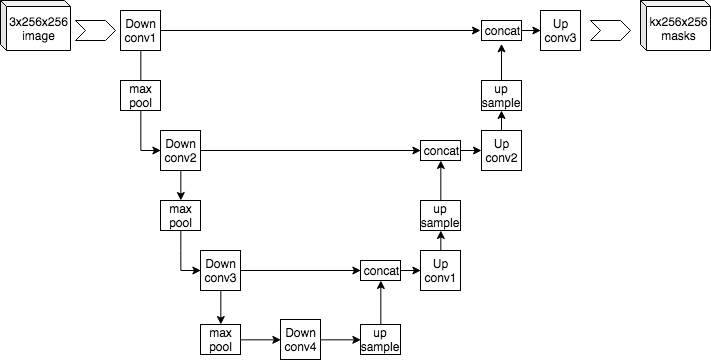
\includegraphics[width=\linewidth]{figures/unet_architecture.png}\\[-0.2em]
    {\small\textbf{(a) U-Net:} encoder, decoder and multi-scale skip connections.}
  \end{minipage}\hfill
  \begin{minipage}[t]{0.48\linewidth}
    \centering
    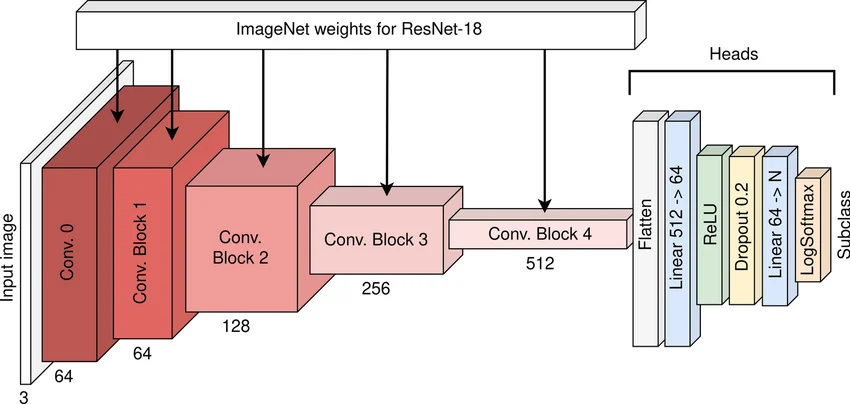
\includegraphics[width=\linewidth]{figures/resnet18_architecture.png}\\[-0.2em]
    {\small\textbf{(b) ResNet18:} residual feature hierarchy and original
    classification heads.}
  \end{minipage}
  \caption{Reference schemes for the two components combined in the implemented model.}
  \label{fig:architectures}
\end{figure}

A ResNet18 pre-trained on ImageNet replaces the original U-Net encoder. Residual blocks
learn a transformation $F(x)$ and add the identity shortcut, producing $F(x)+x$; this
facilitates gradient propagation through the feature extractor. Only the convolutional
stem and the four residual stages are retained. The flattening and classification heads
shown in Figure~\ref{fig:architectures}(b) are discarded, while feature maps with 64,
128, 256 and 512 channels are supplied to the U-Net decoder.

The reference diagrams are generic. In the implemented network, the first ResNet18
convolution is adapted from three RGB channels to one grayscale channel by combining the
pre-trained weights. The decoder ends with a $1\times1$ convolution that returns one
foreground logit per pixel. The complete network has 14.34 million trainable parameters.

\subsection{Input and inference pipeline}

The selected experiment preserves the native $2048^2$ sampling. During training, a
random $1536^2$ crop is extracted from each frame. During inference, four overlapping
$1536^2$ tiles cover the complete image; their probability maps are blended before
thresholding. This procedure keeps native pixel detail while bounding the memory used
by each forward pass.

\begin{center}
\small
\fbox{native grayscale frame}
$\longrightarrow$ \fbox{$1536^2$ train crop / four inference tiles}
$\longrightarrow$ \fbox{ResNet18 U-Net}\\[0.35em]
$\longrightarrow$ \fbox{blended $2048^2$ probabilities}
$\longrightarrow$ \fbox{components}
$\longrightarrow$ \fbox{RLE submission}
\end{center}

Images and masks are decoded once into uint8 memory-mapped files. The cache avoids
repeating JPEG decoding and polygon rasterisation at every epoch without storing the
complete dataset in RAM. It contains only unmodified samples; augmentation is generated
independently at each epoch. During training I apply a random $1536^2$ crop, horizontal
and vertical flips (probability 0.5 each), a random rotation of $0$, $90$, $180$ or
$270$ degrees and photometric perturbations. Brightness and contrast vary within
$\pm20\%$, and Gaussian noise is added in 30\% of the cases. Geometric transforms are
applied to the image and mask together.

\subsection{Optimisation}

For one sample, let $z_j$ be the logit at pixel $j$, $p_j=\sigma(z_j)$ its foreground
probability and $y_j\in\{0,1\}$ the target, over $M$ pixels. The loss terms are:

\begin{samepage}
\begin{itemize}
\item \textbf{Binary Cross-Entropy (BCE):} measures the difference between the
  predicted probability and the target for each pixel, providing local pixel-wise
  supervision.
\item \textbf{Soft Dice loss:} measures the overlap between predicted and ground-truth
  masks. It is useful under strong foreground-background imbalance because it directly
  considers the area of the two regions.
\item \textbf{Combined loss:} averages the two terms, assigning weight 0.5 to each.
\end{itemize}
\end{samepage}

The definitions used are
\begin{equation}
\begin{aligned}
\mathcal{L}_{\mathrm{BCE}}
  &= -\frac{1}{M}\sum_{j=1}^{M}\left[y_j\log(p_j)+(1-y_j)\log(1-p_j)\right],\\
\mathcal{L}_{\mathrm{Dice}}
  &= 1-\frac{2\sum_{j=1}^{M}p_jy_j+\varepsilon}
  {\sum_{j=1}^{M}p_j+\sum_{j=1}^{M}y_j+\varepsilon},\quad \varepsilon=10^{-6},\\
\mathcal{L} &= 0.5\,\mathcal{L}_{\mathrm{BCE}}+0.5\,\mathcal{L}_{\mathrm{Dice}}.
\end{aligned}
\end{equation}
The stabilising constant $\varepsilon$ avoids a zero denominator, and both terms are
averaged over the mini-batch.
No positive-class weight is used in experiment 13. AdamW is configured with learning
rate $10^{-4}$, weight decay $10^{-4}$ and cosine decay over at most 20 epochs.
Checkpoint selection and early stopping are based on validation Dice; the saved
checkpoint is epoch \finalepoch.

The effective batch size is 2. One crop is processed at a time and gradients are
accumulated over two forward/backward passes. Gradient checkpointing and bfloat16 mixed
precision are also enabled. The training stopped after 15 epochs and required
\finaltrainmemory{} at peak; inference required \finaltestmemory{}.

Finally, the probability map is converted into connected components using the operating
point selected on validation. The final values and the distinction between Dice- and
PQ-oriented configurations are reported in Section~\ref{sec:results}.
